\chapter{Results}
\label{cha:results}

\section{Final Distribution}
\label{sec:final-dist}

Having accounted for the systematic uncertainties, one can examine the final distribution(s). This encompasses the mass of the gaugino and smuon. In case of the smuon, the selected two jets and the two muons enter the invariant mass calculation. Removing the leading muon from this composition yields the gaugino case. All event selection requirements are applied and in relation to the control region BVC, only the inverted missing transverse energy requirement is reversed again $E_{\text{T}}^{\text{miss}} < 50\,\text{GeV}$. Figure~\ref{fig:final-dist} shows both distributions including the data-driven background estimate.

\begin{figure}[htb!]
  \centering
  \begin{subfigure}[b]{0.495\textwidth}
    \centering
    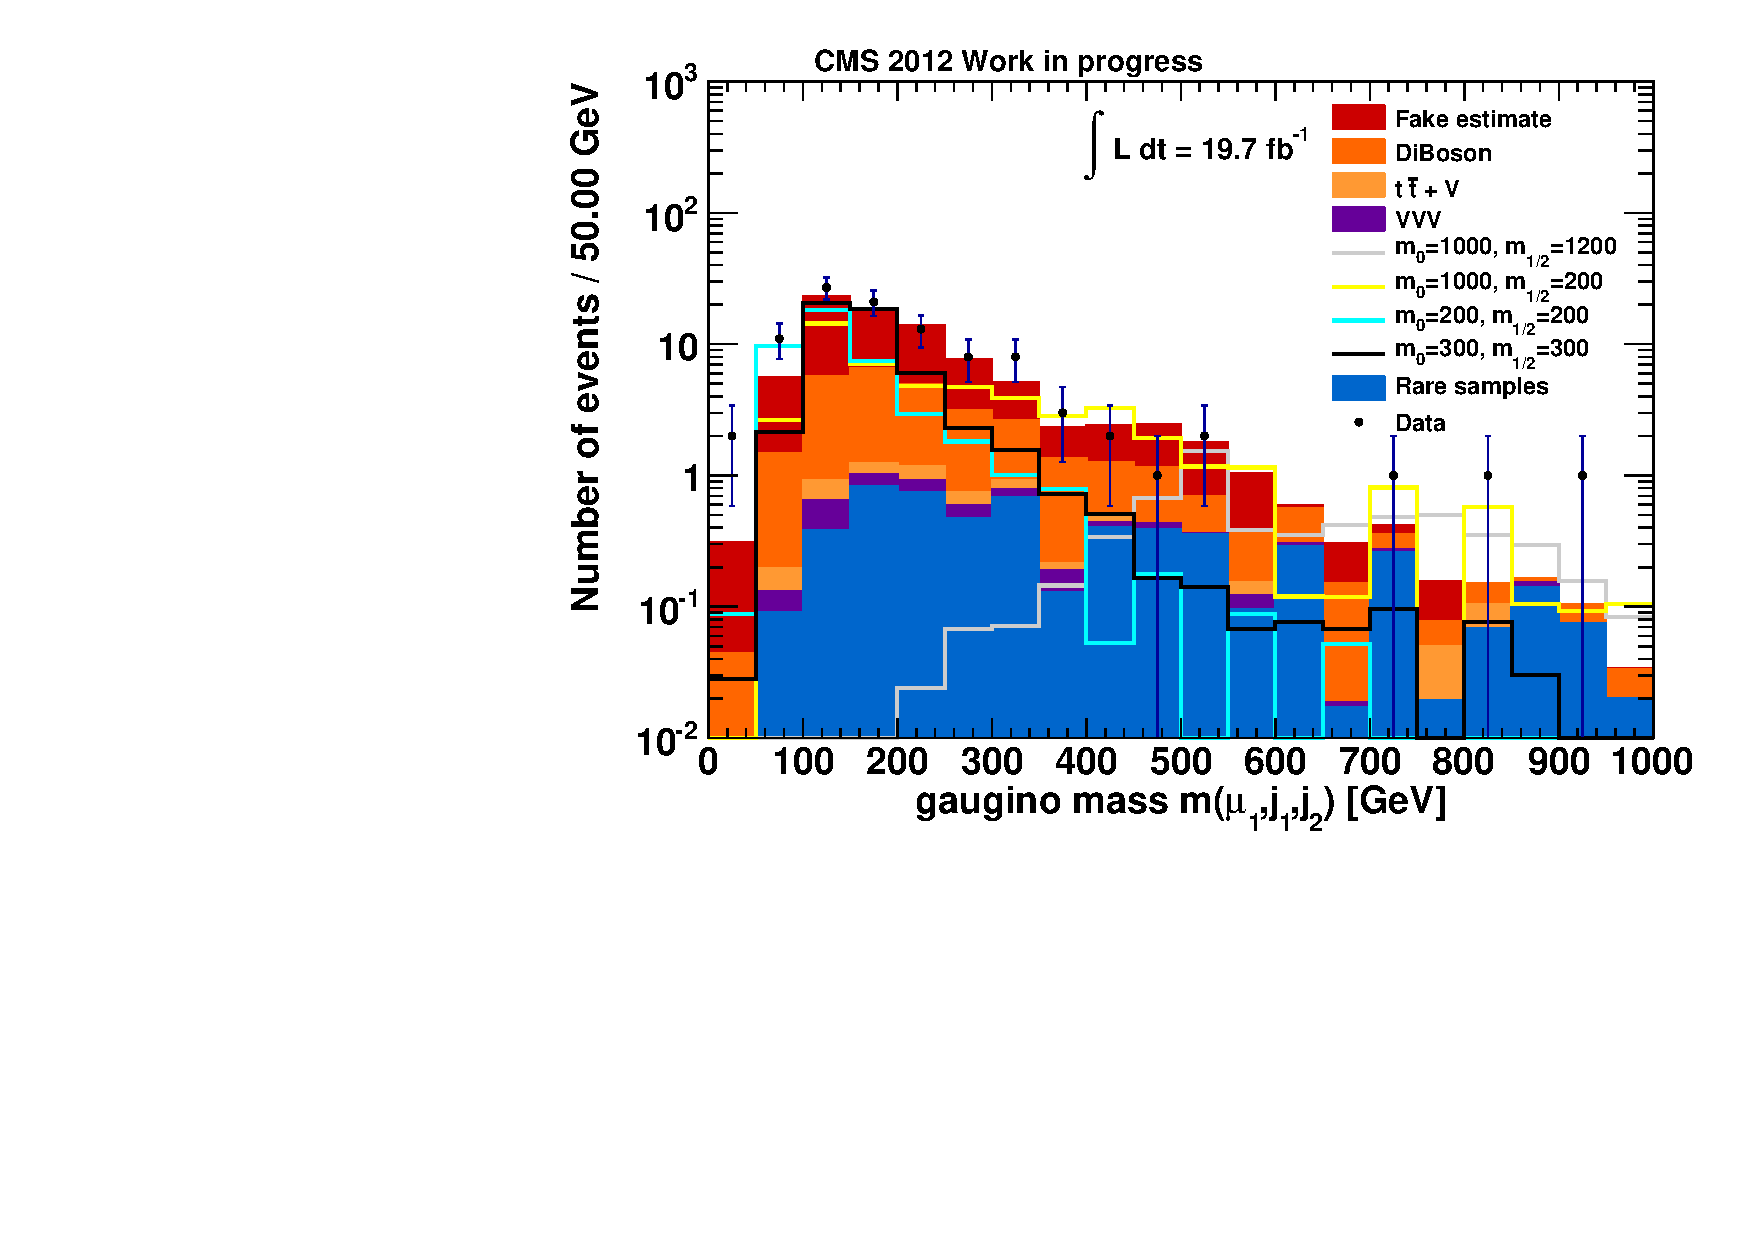
\includegraphics[width=\textwidth]{plots/m_gaugino.pdf}
    \caption{\label{fig:m_gaugino}}
  \end{subfigure}
  \begin{subfigure}[b]{0.495\textwidth}
    \centering
    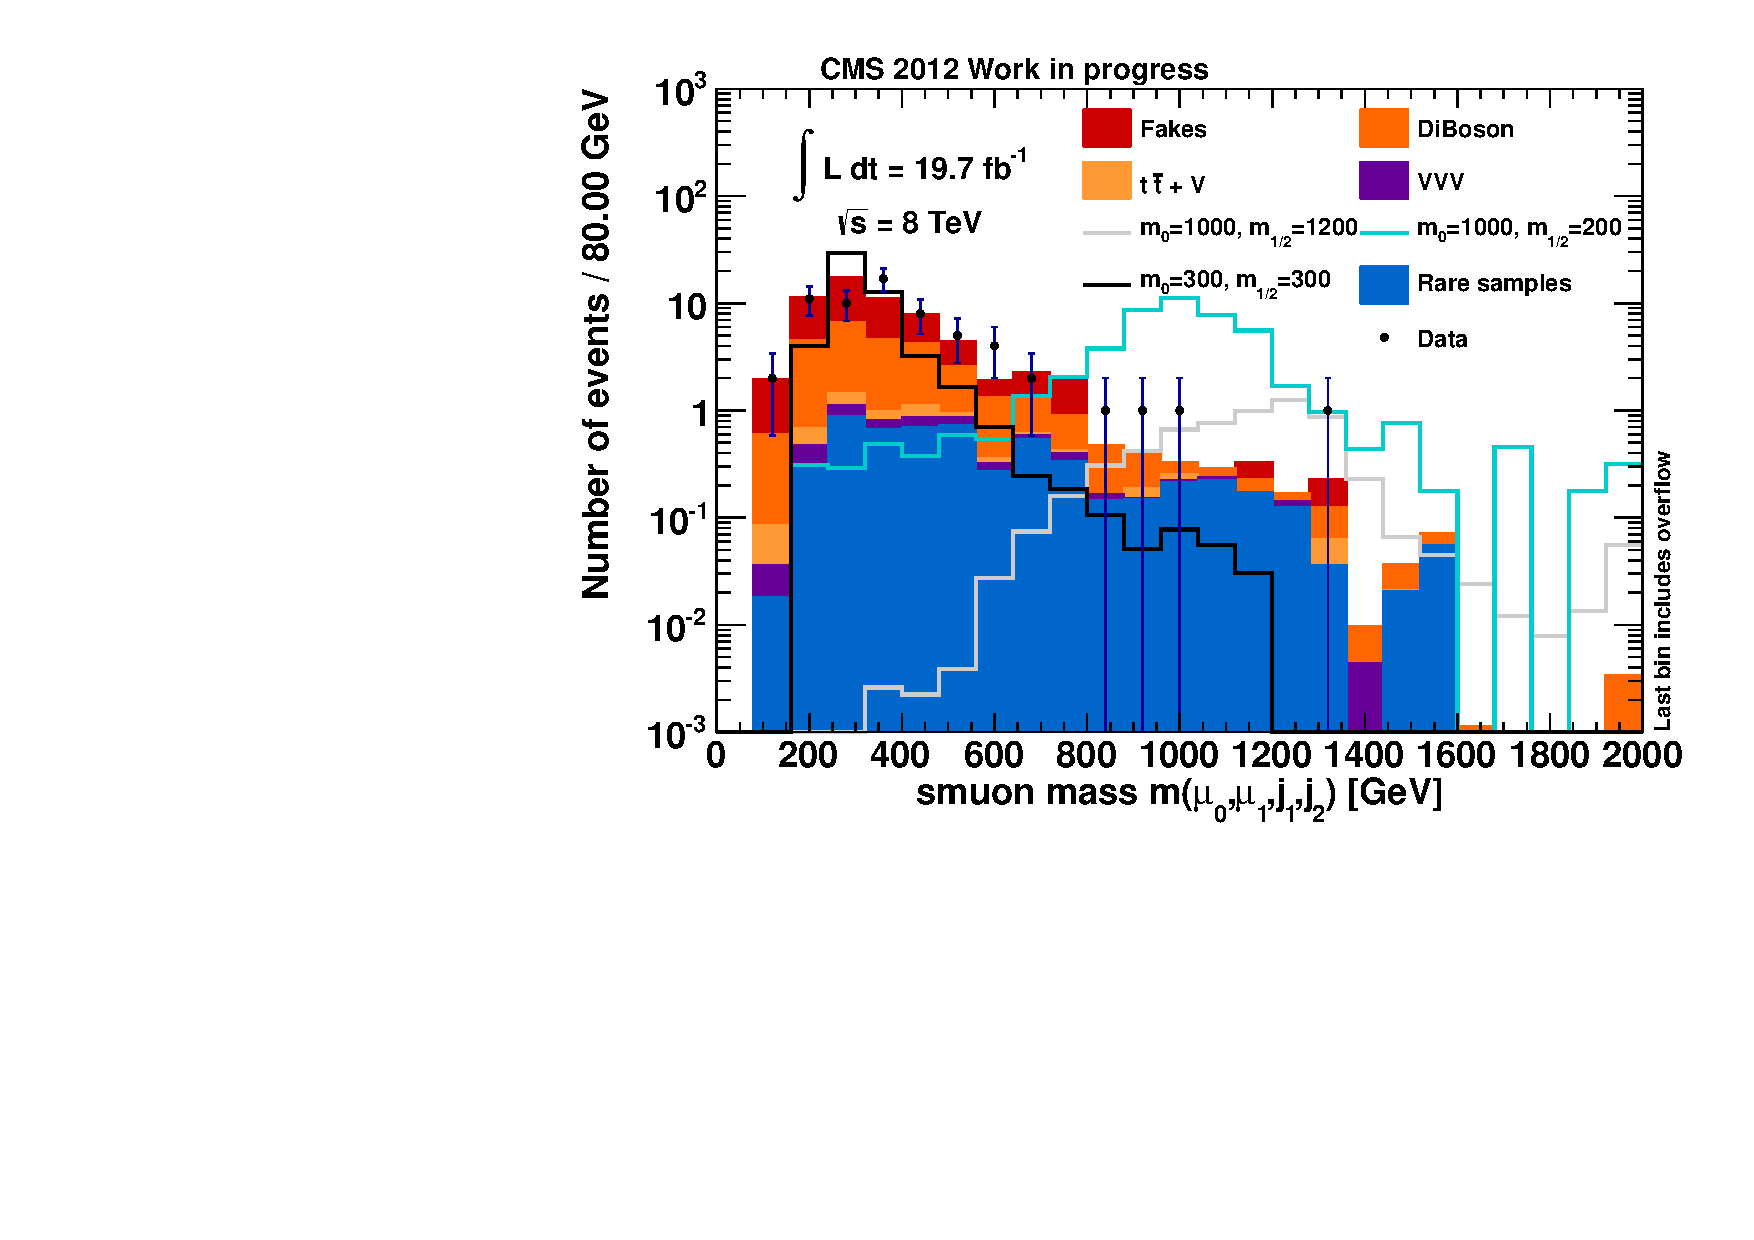
\includegraphics[width=\textwidth]{plots/m_smuon.pdf}
    \caption{\label{fig:m_smuon}}
  \end{subfigure}
  \caption{Mass of the gaugino (\ref{fig:m_gaugino}) and smuon (\ref{fig:m_smuon}). Both are calculated from the invariant masses of the selected two jets and two muons in the smuon case, as well as two jets and the sub leading muon for the gaugino. The distributions include the data-driven background estimate.}
  \label{fig:final-dist}
\end{figure}

\noindent Table~\ref{tab:nev-msmuon} resolves each group of processes into its individual background components. The importance of the data-driven background estimate is shown by its large contribution. Combined with the $WZ \rightarrow 3l \nu$ process, it adds up to more than $80\,\pct$ of the entire background prediction.

\begin{table}[!htb]
  \centering
  \begin{tabular}{|l|c|c|c|}
    \hline
    \multirow{2}{*}{Backgrounds}    & \multirow{2}{*}{$N_{\text{Events}}$} & \multicolumn{2}{|c|}{Uncertainties} \\ \cline{3-4}
                                    &                                      & stat.  & sys.                       \\ \hline \hline
    Fake estimate                   & 33.5                                 & 2.4    & 16                         \\ \hline
    $W\gamma \rightarrow l\nu 2\mu$ & 1.35                                 & 0.45   & 0.69                       \\
    $WZ \rightarrow 3l \nu$         & 17.1                                 & 0.5    & 1.9                        \\
    $WZ \rightarrow 2q l \nu$       & 0.026                                & 0.026  & 0.003                      \\
    $ZZ \rightarrow 2l 2q$          & 0.044                                & 0.030  & 0.0044                     \\
    $ZZ \rightarrow 4l$             & 2.55                                 & 0.05   & 0.27                       \\ \hline
    $t\bar{t} + W$                  & 1.0                                  & 0.16   & 0.30                       \\
    $t\bar{t} + WW$                 & 0.0163                               & 0.0019 & 00083                      \\
    $t\bar{t} + Z$                  & 0.258                                & 0.070  & 0.038                      \\ \hline
    $WWW$                           & 0.842                                & 0.081  & 0.085                      \\
    $WWZ$                           & 0.186                                & 0.034  & 0.02                       \\
    $WZZ$                           & 0.186                                & 0.013  & 0.001                      \\
    $ZZZ$                           & 0.0554                               & 0.0018 & 0.0005                     \\ \hline
    $W^- W^-$                       & 1.38                                 & 0.17   & 0.7                        \\
    $W^+ W^+$                       & 3.97                                 & 0.48   & 2.02                       \\
    $WW$ Double-parton              & 0.24                                 & 0.07   & 0.12                       \\ \hline
    $\sum$                          & 62.5                                 & 2.6    & 22.1                       \\ \hline
    Data                            & 63                                   & -      & -                          \\ \hline
  \end{tabular}
  \caption{Detailed number of events for each background in the distributions at the final stage of the analysis.}
  \label{tab:nev-msmuon}
\end{table}

The statistical uncertainties for the Monte Carlo predictions stem from the generated number of events, which limit the accuracy of the prediction. While the fake estimate has been determined from data, the method itself inherits said statistical uncertainties as some background samples are subtracted from the data when determining the tight-to-loose ratio. Respectively adding the uncertainties for every bin of the single- and double-fake estimates in quadrature and propagating them according to equation~\eqref{eq:fakes}, yields the statistical uncertainty for this case. All systematic uncertainties are taken from the summary table (Tab.~\ref{tab:sys-uncertainties}). Individual cross section uncertainties are included in accordance to the table's description as well. Overall one can observe an excellent agreement of measurement and SM simulation. All variations are well within the given uncertainties.

Taking the signal point with $m_0 = 1000\,\text{GeV}$ and $m_{1/2} = 200\,\text{GeV}$ in figure~\ref{fig:final-dist} as an example, one can see that while the distributions coincide in the gaugino mass distribution, they do not in the smuon one. To improve the results a multi-bin approach is being employed. For that purpose the two dimensional gaugino-smuon mass distribution is divided into six regions, which is shown in figure~\ref{fig:m_smu_chi}.

\begin{figure}[!htb]
  \centering
  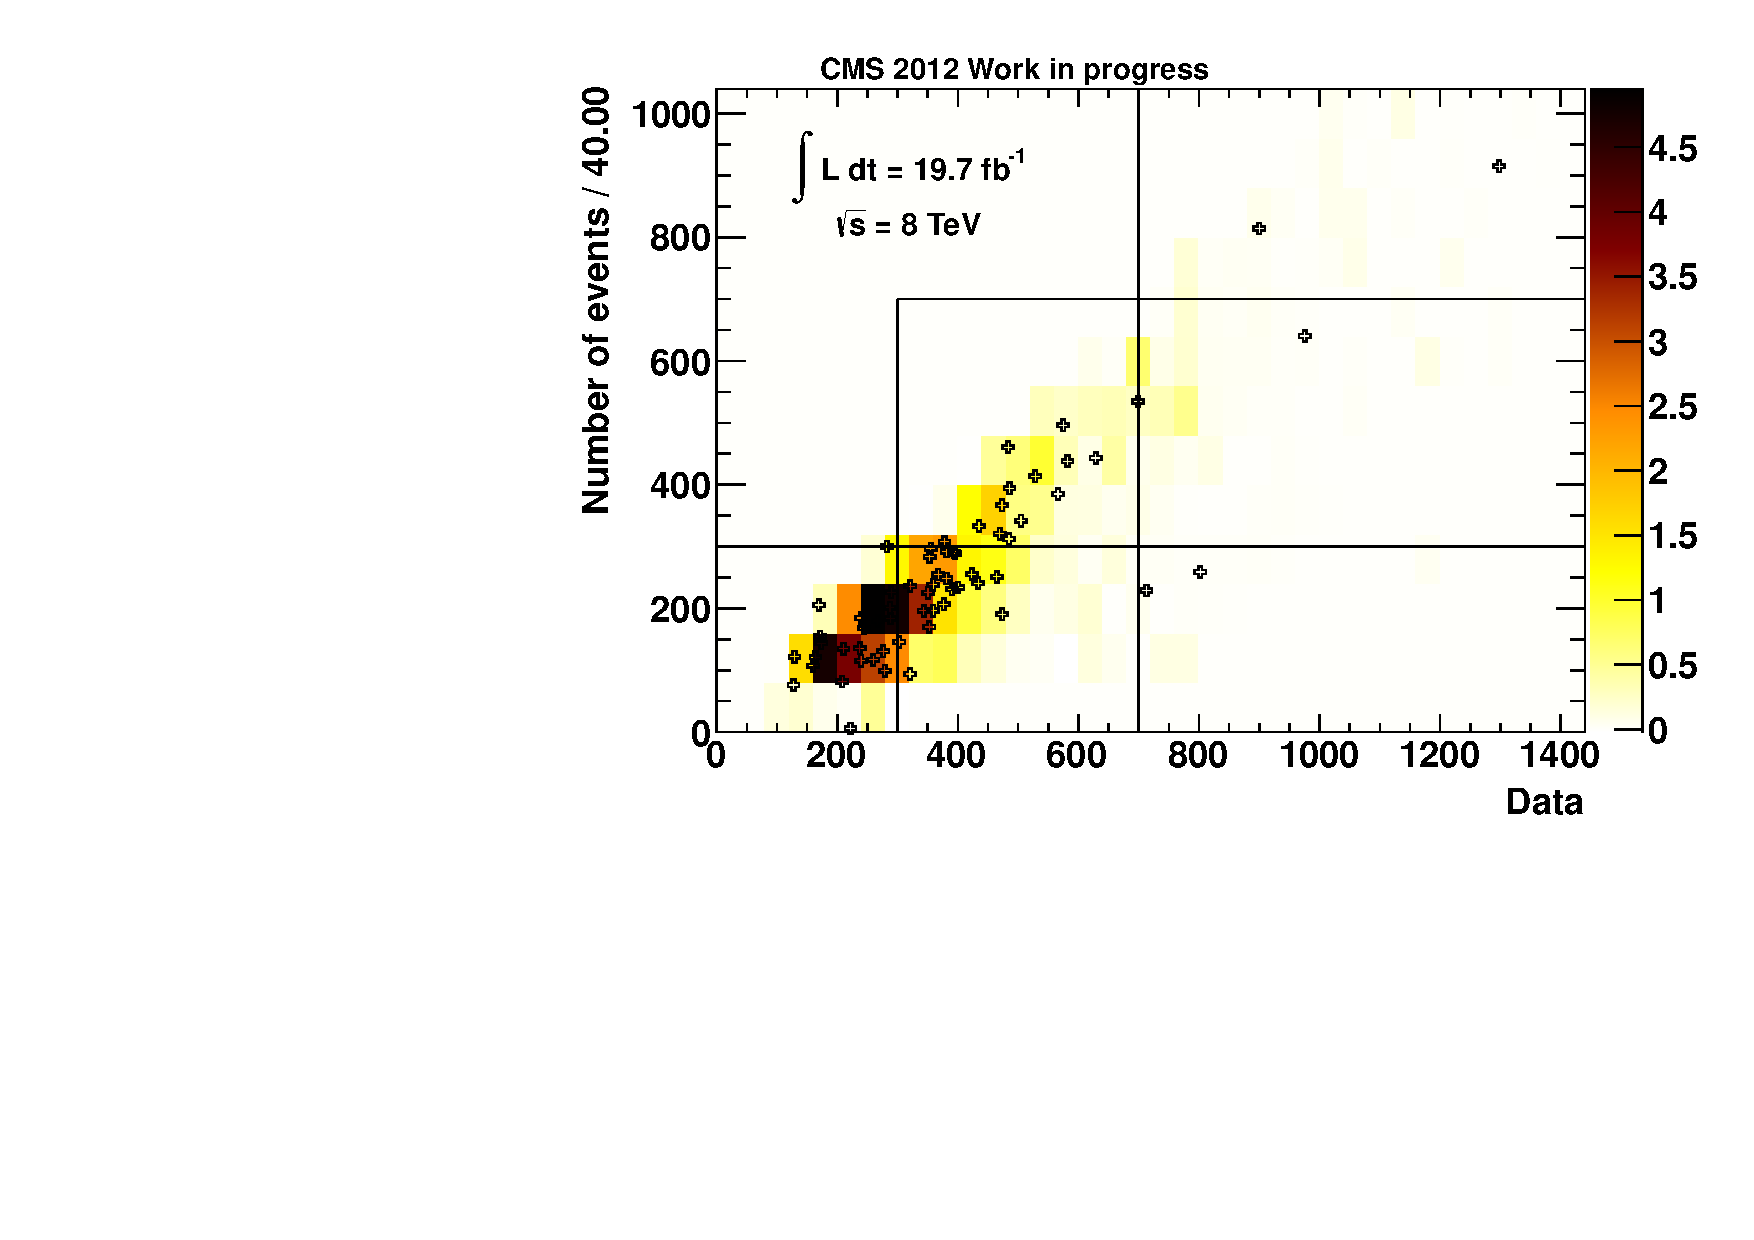
\includegraphics[width=0.7\textwidth]{plots/m_smu_chi.pdf}
  \caption{Two-dimensional smuon and gaugino mass distribution. All backgrounds are summed up and are shown as coloured signal regions, while the data points are shown individually. The six bins are regarded as separate signal regions to improve the results of this analysis.}
  \label{fig:m_smu_chi}
\end{figure}

\noindent Most entries are centered around one diagonal line. In comparison, the aforementioned signal point has the majority of its entries at smuon masses above $1200\,\text{GeV}$. The contents of each of the six regions, are summarized in table~\ref{tab:m_smu_chi_summary}.

\begin{table}[!htbp]
  \centering
  \begin{tabular}{|l|r|r|r|}
    \hline
    Process group & SR 1              & SR 2              & SR 3              \\ \hline
    Fakes         & 16.0 $\pm$ 1.63   & 10.7 $\pm$ 1.3    & 5.00 $\pm$ 0.98   \\ 
    $tt+V$        & 0.47 $\pm$ 0.10   & 0.49 $\pm$ 0.11   & 0.187 $\pm$ 0.068 \\ 
    $VV$          & 8.46 $\pm$ 0.40   & 7.10 $\pm$ 0.40   & 4.01 $\pm$ 0.29   \\
    $VVV$         & 0.374 $\pm$ 0.051 & 0.392 $\pm$ 0.052 & 0.209 $\pm$ 0.040 \\ 
    Rare          & 1.04 $\pm$ 0.21   & 1.33 $\pm$ 0.24   & 1.65 $\pm$ 0.28   \\ \hline
    $\sum$        & 26.4 $\pm$ 9.6    & 20.0 $\pm$ 7.1      & 11.1 $\pm$ 4.0    \\ \hline
    Data          & 19                & 25                & 13                \\ \hline \hline
    Process group & SR 4                & SR 5              & SR 6              \\ \hline
    Fakes         & 0.23 $\pm$ 0.16     & 1.15 $\pm$ 0.69   & 0.33 $\pm$ 0.19   \\
    $tt+V$        & $<0.001 \pm <0.001$ & 0.032$\pm$ 0.027  & 0.094 $\pm$ 0.054 \\
    $VV$          & 0.106 $\pm$ 0.032   & 1.07 $\pm$ 0.11   & 0.277 $\pm$ 0.054 \\
    $VVV$         & 0.0062 $\pm$ 0.0047 & 0.090 $\pm$ 0.026 & 0.028 $\pm$ 0.014 \\
    Rare          & 0.102 $\pm$ 0.072   & 0.65 $\pm$ 0.17   & 0.80 $\pm$ 0.21   \\ \hline
    $\sum$        & 0.45 $\pm$ 0.25     & 3.0 $\pm$ 1.3     & 1.5 $\pm$ 0.7     \\ \hline
    Data          & 2                   & 1                 & 3                 \\ \hline
  \end{tabular}
  \caption{Summary of the six regions displayed in figure~\ref{fig:m_smu_chi}. They are numbered starting on the left and progressing upwards from the lowest bin.}
  \label{tab:m_smu_chi_summary}
\end{table}

\section{Calculation of Limits}
\label{sec:calc-of-limits}

As any excess of data is too slight to be considered statistically significant, one can translate the result into limits onto two quantities. The cross section of a RPV SUSY model and its model parameters. To calculate these, the method commonly used amongst the CMS experiment will be utilized. Details are given in the upcoming section.


\subsection{CLs Method}
\label{sec:cls-method}

To complement Bayesian and common frequentist methods, the $CL_s$ method~\cite{cls,cls2} has been developed. It is considered a modified frequentist analysis. Compared to the former two, its results are better in cases with low statistics and are less background dependent. The general idea is to compare two hypotheses to a measurement.

% Confidence levels are defined as the probability of the respective hypothesis to describe the measured data.

For most analyses in high energy particle physics, there are two cases to be covered. The null hypotheses $H_0$ being the Standard Model prediction by itself and a combination of the proposed signal and the Standard Model prediction as the second hypothesis $H_1$. In the most simple case, given enough statistics, one expects the number of events $n$ to follow a Poisson distribution.

\begin{equation}
  \label{eq:poisson-likelihood}
    \mathcal{L} (x; n) = \frac{x^n}{n!} e^{-x}
\end{equation}

\noindent These likelihoods $\mathcal{L}_x$ are the basis for this method. Here, $x$ denotes the background-only scenario for $x = b$ and the background plus signal one for $x = s + b$. The distributions are ultimately a function of the cross section of the relevant processes, as it proportional to the number of selected events $n$.

Using the two likelihoods, a test statistic $Q$ can be defined. It is called the \textit{likelihood-ratio} and is used to judge how well a hypothesis describes the measurement. In the most simple case, it is given by

\begin{equation}
  \label{eq:testq}
  Q = \frac{\mathcal{L} (s + b; n)}{\mathcal{L} (b; n)}.
\end{equation}

\noindent Large values of $Q$ correspond to a better agreement with $H_1$, while small ones to a better agreement with $H_0$. For a result of an actual experiment, the observed number of events $n_{\text{obs}}$ yields a set likelihood-ratio $Q_{\text{obs}}$.

The confidence level for either hypothesis to be an accurate description for $Q_{\text{obs}}$, is given as

\begin{equation}
  \label{eq:cl-prob}
  CL_x = P (Q \leq Q_{obs}).
\end{equation}

\noindent Here, $P$ denotes the probability for a test statistic $Q$ being less or equal to the observed statistic $Q_{\text{obs}}$. It is determined through integration.

\begin{equation}
  \label{eq:clx}
  CL_x = \int^{Q_{\text{obs}}}_{-\infty} \frac{d f_x(Q)}{d Q} \text{d} Q
\end{equation}

\noindent The probability distribution functions are denoted by $f_x(Q)$ and are usually determined through pseudo-experiments. For a very well understood background hypothesis, a confidence level in the null hypothesis of $CL_b (Q_{\text{obs}}) \approx 1$ is necessary to claim a discovery. The specific thresholds that $1 - CL_b (Q_{\text{obs}})$ has to fall below, are derived from the Gaussian distribution. This means $2.7 \cdot 10^{-3}$ corresponds to $3\,\sigma$, which is considered ``evidence'', and $5.7 \cdot 10^{-5}$ corresponding to $5\,\sigma$, a discovery.

Excluding the signal (plus background) hypothesis uses the eponymous $CL_s$ quantity instead of $CL_{s+b}$. It is defined as a ratio:

\begin{equation}
  \label{eq:cls}
  CL_s = \frac{CL_{s+b}}{CL_b}.
\end{equation}

\noindent While $CL_{s+b}$ may lead to unphysical results in certain cases, $CL_s$ does not. A prime example is a signal hypothesis that is dominated by its background. Slight fluctuations towards lower values of the latter would lead to a very low $CL_{s+b}$, yielding a strong exclusion limit. As $CL_s$ is not a confidence limit, but a ratio of those, fluctuations like these cancel themselves out.

A signal can be excluded to a confidence level $CL$, when the following relation is fulfilled.

\begin{equation}
  \label{eq:cl-excl}
  1 - CL_s \leq CL
\end{equation}

\section{Modifications}
\label{sec:mods}

Following the recommendations by the CMS and ATLAS collaborations~\cite{clsmod}, a modified test statistic is employed for the $CL_s$ method. To scale the signal strength, a parameter $\mu$ is introduced to the formula. It is used to in- or decrease the cross section of the signal prediction while the branching ratios remain constant. Additionally, both the signal and background simulation are subject to a number of uncertainties. To account for those in the limit calculation, a set of nuisance parameters $\theta$ is introduced.

\begin{equation}
  \label{eq:q-mod}
  Q = - 2 \ln{ \frac{\mathcal{L} (\mu s + b; n, \hat{\theta)_\mu}) }{\mathcal{L} (\hat{\mu} \cdot s + b; n, \hat{\theta} )} } \quad \text{ with } \quad 0 \leq \hat{\mu} \leq \mu
\end{equation}

\noindent Here, the pair of parameters $\hat{\mu}$ and $\hat{\theta}$ are evaluated at the global maximum of the likelihood. $\hat{\theta}_\mu$ on the other hand denotes the conditional maximum likelihood estimator of $\theta$, which also depends on the choice of $\mu$.

% Using the logarithm with a factor of $-2$ allows the test statistic to converge against $\Delta \chi^2$ for a large number of selected events.

To improve the limits, the signal region is subdivided into multiple signal regions. When combining the results for the individual regions, the respective likelihoods have to be multiplied and the overall value is given by

\begin{equation}
  \label{eq:likelihood-product}
  \mathcal{L} = \prod_i \mathcal{L}_i.
\end{equation}

\noindent This enhances the sensitivity, as the influence of large deviations in one region is increased.

\section{Limit Graphs}
\label{sec:limit-graphs}

The actual calculation of limits is performed by the \textsc{HiggsCombine} tool~\cite{clsmod,higgscombine}. It employs the \textsc{RooStats} package~\cite{roostats} which is part of the statistical analysis framework \textsc{ROOT}. In line with all CMS publications, the exclusion ranges are calculated at a $95\,\pct$ confidence level as a upper limit on the cross section ($CL_s \leq 0.05$). The necessary scaling of the signal strength to reach this $CL$ can be achieved through varying the previously introduced modifier $\mu$. This has to be done for each of the individual points in the RPV SUSY phase space.

While the result of the calculation is a limit on the signal cross section $\sigma$, it can be translated into a limit onto the model parameter $\lambda^\prime_{211}$. As the former scales quadratically with the latter, the following formula has to be used.

\begin{equation}
  \label{eq:xs-lambda-scale}
  \sigma \propto \lambda^{\prime\:2}_{211} \Rightarrow \lambda^\prime_{211} (95\,\pct\: CL) = \lambda^\prime_{211} \cdot \sqrt{ \frac{\sigma (95\,\pct\: CL)}{\sigma} } 
\end{equation}

The respective $95\,\pct\: CL$ multi-bin upper cross section limits, which have been translated into limits on the model parameter $\lambda^{\prime}_{211}$ are displayed as a function of $m_0$ and $m_{1/2}$ in figure~\ref{fig:lambda-prime-limits} and as a function of $m_{\tilde{\mu}}$ and $m_{\tilde{\chi}^0}$ in this RPV model in figure~\ref{fig:smu-nt0-limits}. One should note that, while $m_{\tilde{\chi}^0}$ corresponds to the LSP right before its RPV decay, $m_{\tilde{\mu}}$ represents the initial supersymmetric particle. Consequently, the sneutrino case $m_{\tilde{\nu}}$ is also included. As explained in the signal study (Cha.~\ref{cha:sig}), the LSP might be the product of prior RPC decays from the smuon, instead of being a direct decay product. With this in mind, one has to be careful when interpreting the latter two limit graphs.

\begin{figure}[!htbp]
  \centering
  \begin{subfigure}[b]{0.85\textwidth}
    \centering
    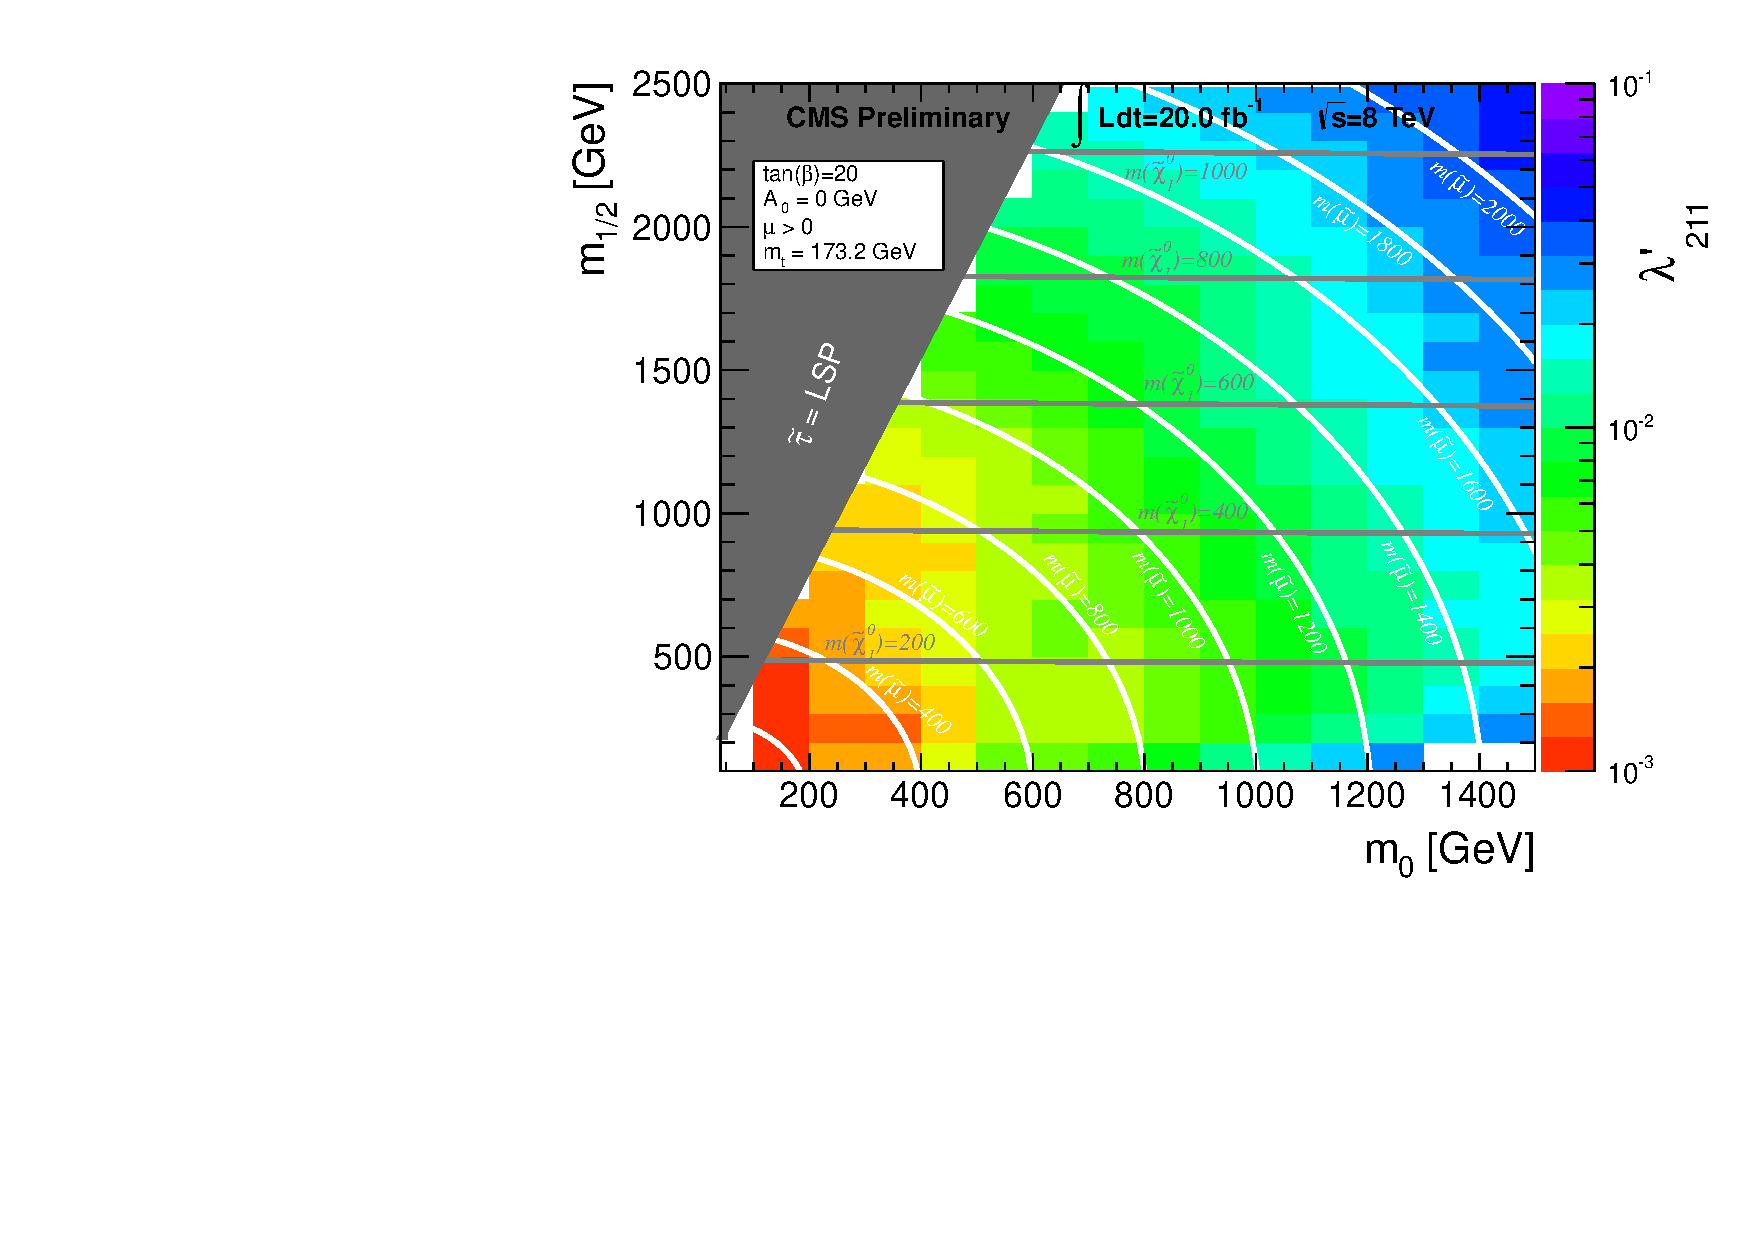
\includegraphics[width=\textwidth]{plots/l211limits_MultiBin_expected_logz-colz.pdf}
    \caption{\label{fig:lambda-prime-exp}}
  \end{subfigure}
  \begin{subfigure}[b]{0.85\textwidth}
    \centering
    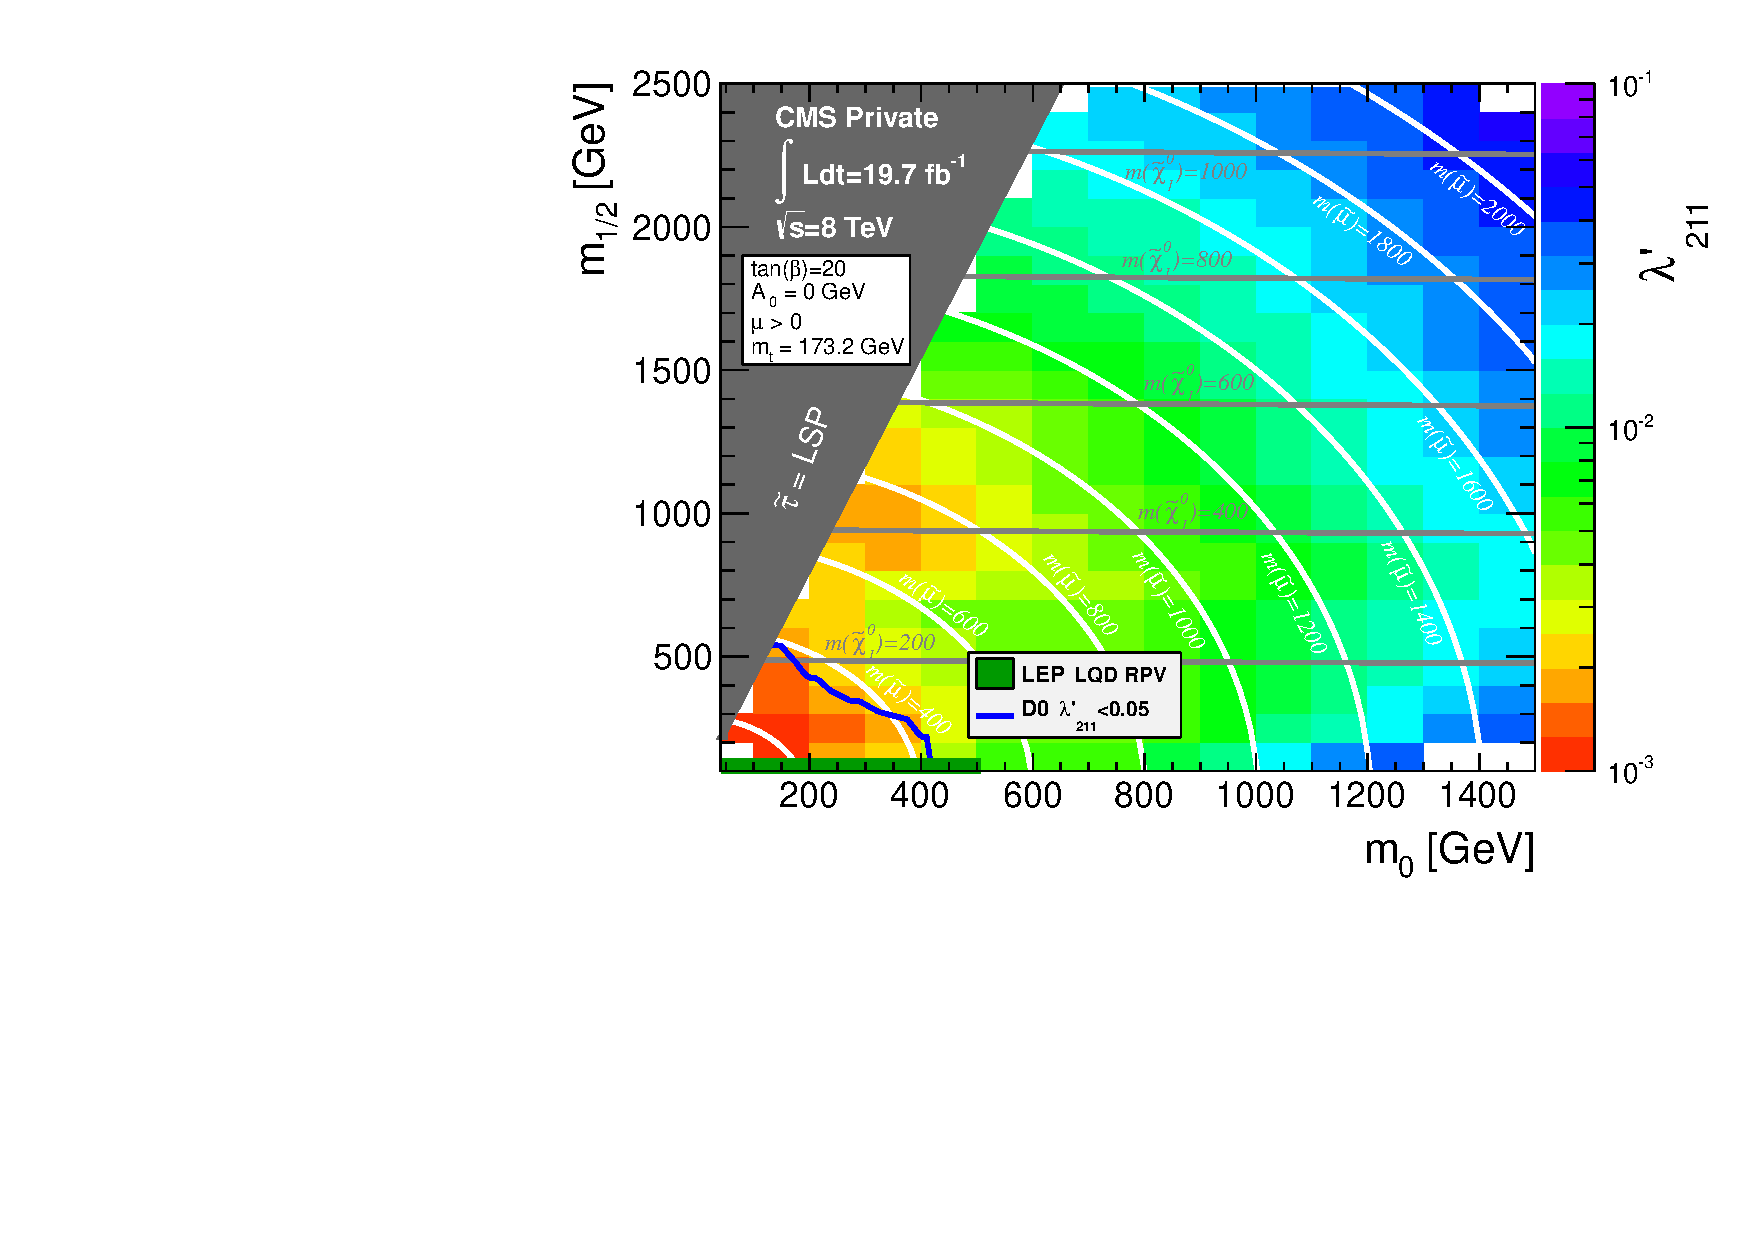
\includegraphics[width=\textwidth]{plots/l211limits_MultiBin_logz-colz.pdf}
    \caption{\label{fig:lambda-prime-obs}}
  \end{subfigure}
  \caption{Expected (\ref{fig:lambda-prime-exp}) and observed (\ref{fig:lambda-prime-obs}) $95\,\%\: CL$ upper limits on the $\lambda^{\prime}_{211}$ coupling. They are given as a function of $m_0$ and $m_{1/2}$, while $A_0 = 0\,\text{GeV}$, $\text{sgn}(\mu) = +1$ and $\tan{\beta} = 20$.}
  \label{fig:lambda-prime-limits}
\end{figure}

\begin{figure}[!htbp]
  \centering
  \begin{subfigure}[b]{0.90\textwidth}
    \centering
    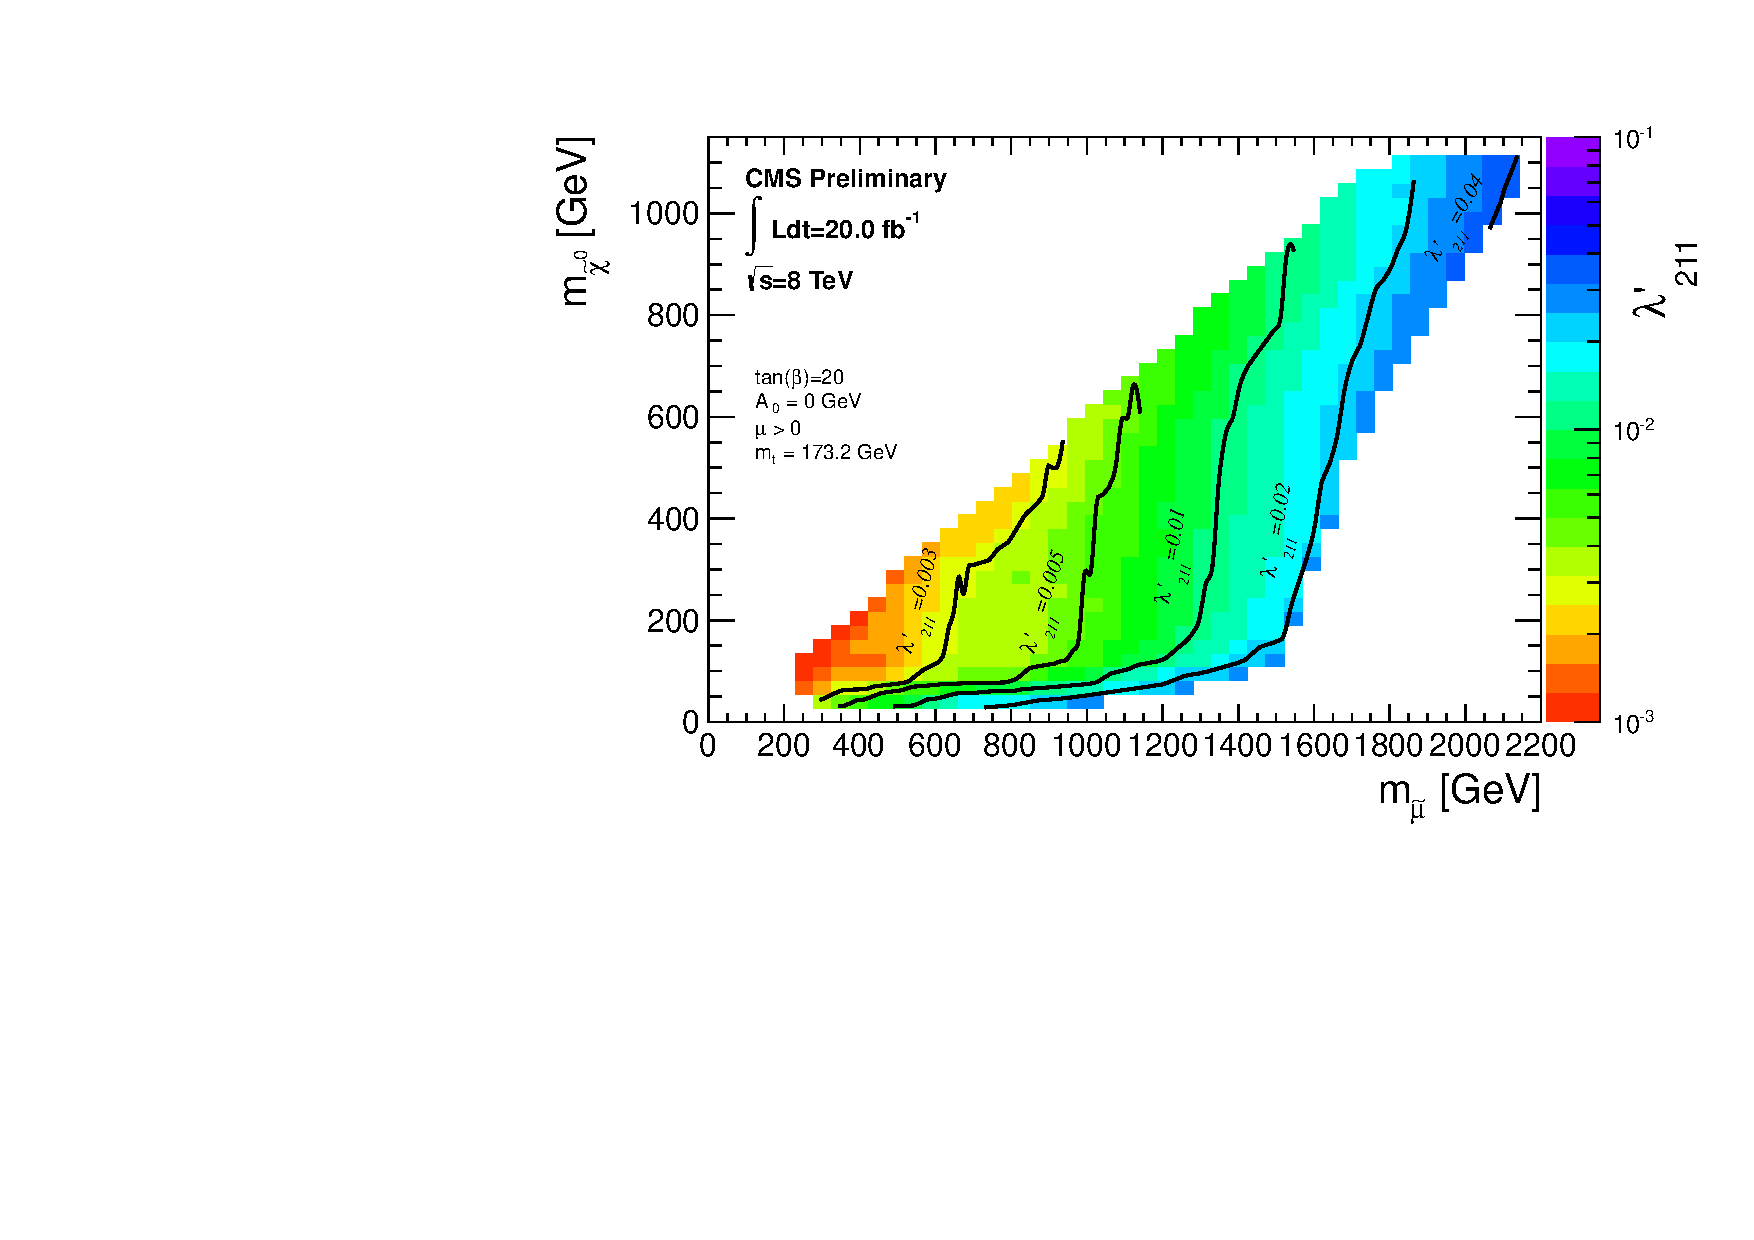
\includegraphics[width=\textwidth]{plots/plot_smuon_neutralino_mass_expectedLimitsCombine.pdf}
    \caption{\label{fig:m-smu-nt0-exp}}
  \end{subfigure}
  \begin{subfigure}[b]{0.90\textwidth}
    \centering
    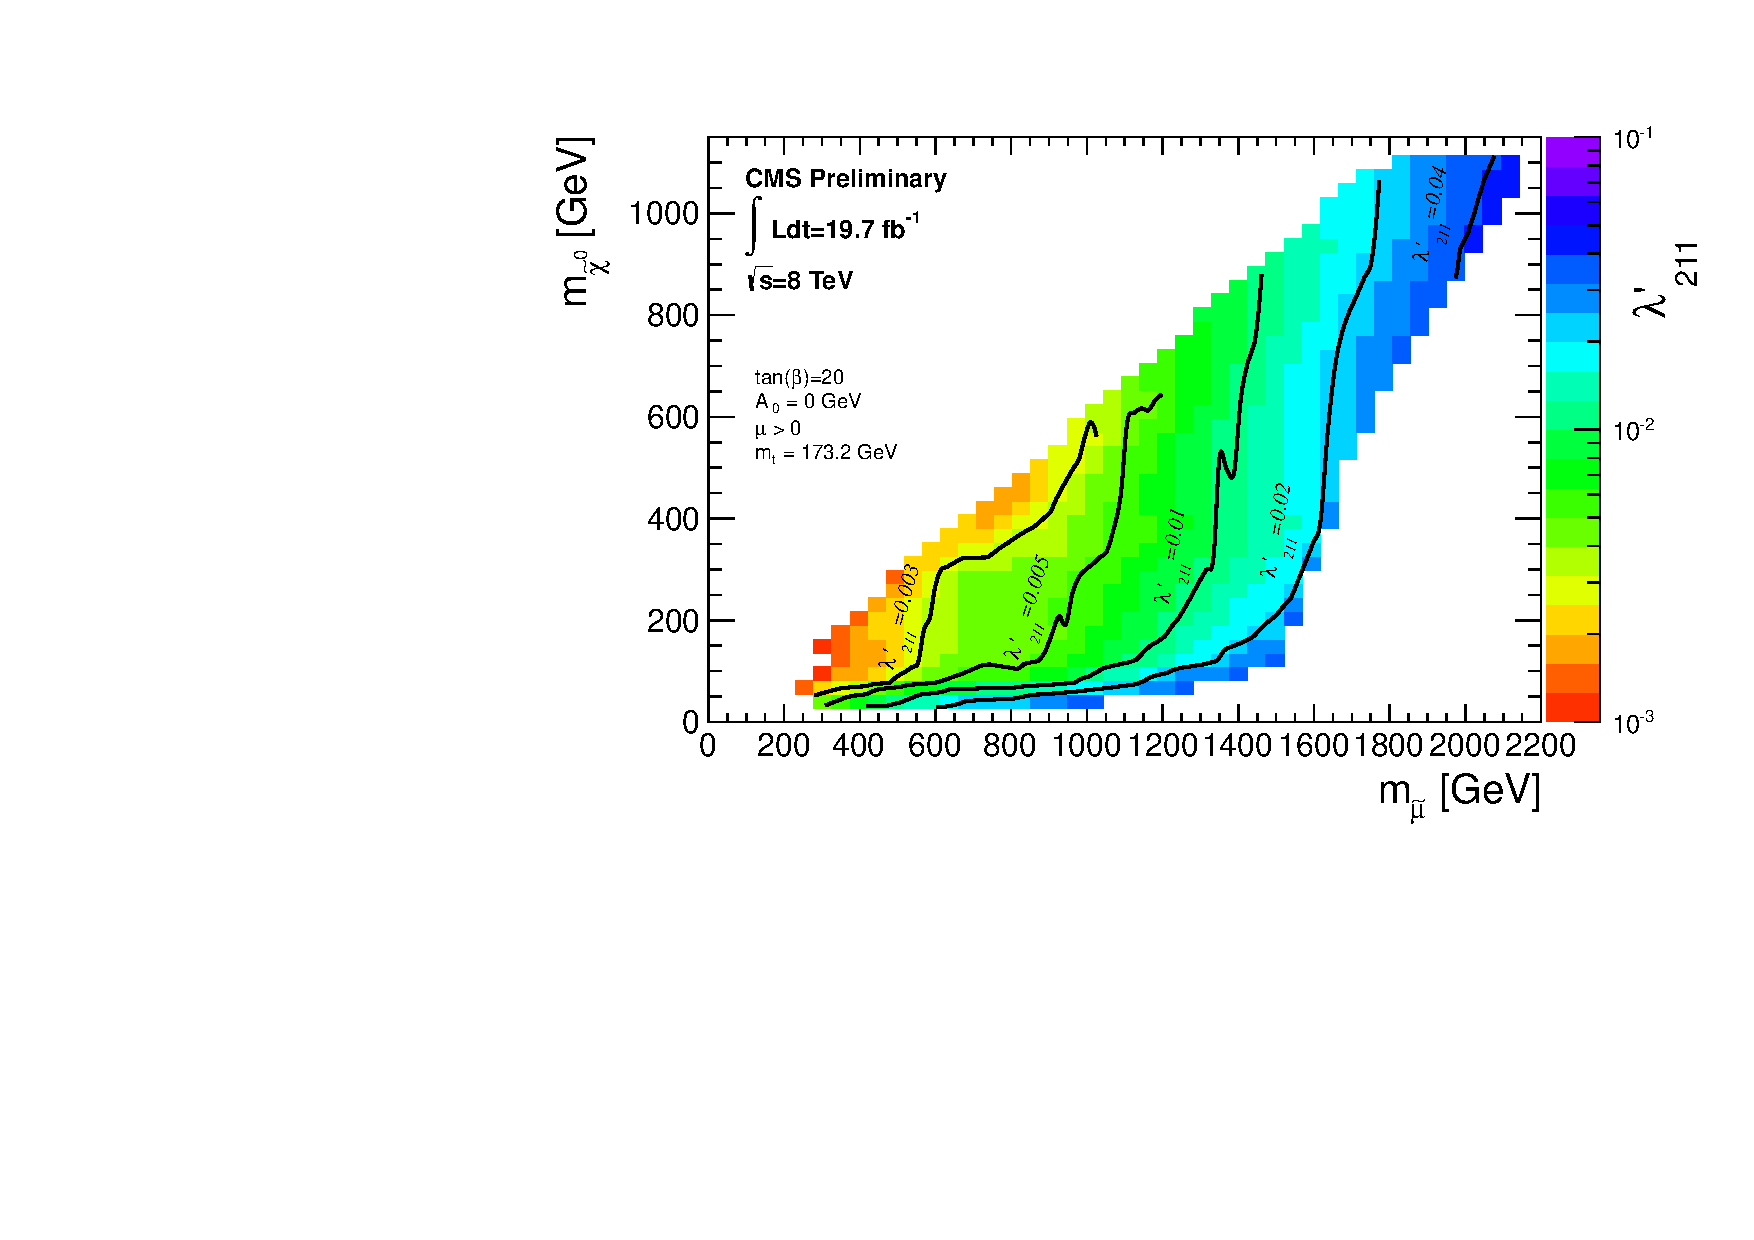
\includegraphics[width=\textwidth]{plots/plot_smuon_neutralino_mass_LimitsCombine.pdf}
    \caption{\label{fig:m-smu-nt0-obs}}
  \end{subfigure}
  \caption{Expected (\ref{fig:m-smu-nt0-exp}) and observed (\ref{fig:m-smu-nt0-obs}) $95\,\%\: CL$ upper limits on the $\lambda^{\prime}_{211}$ coupling. They are given as a function of $m_{\tilde{\mu}}$ and $m_{\tilde{\chi}^0}$, while $A_0 = 0\,\text{GeV}$, $\text{sgn}(\mu) = +1$ and $\tan{\beta} = 20$.}
  \label{fig:smu-nt0-limits}
\end{figure}


\section{Discussion and Thoughts}
\label{sec:discussion}

Comparing the shown limits to the analyses of 2011 RPV SUSY and the D0 predecessor, the phase space that is being covered has been expanded considerably. The simulation with the highest universal mass parameters for D0 was $m_0 = 500\,\text{GeV}$, $m_{1/2} = 600\,\text{GeV}$, while it had increased to $m_0 = 1300\,\text{GeV}$, $m_{1/2} = 1000\,\text{GeV}$ in the 2011 CMS analysis. With the given results, it now lies at $m_0 = 1500\,\text{GeV}$, $m_{1/2} = 2500\,\text{GeV}$. In addition to that, the excluded values of $\lambda^{\prime}_{211}$ are roughly a factor of 10 better than the ones presented by D0~\cite{auter,d0rpv}, and around a factor of 1.8 in regards to the 2011 analysis~\cite{2011rpv}. One can base a rough evaluation of this improvement off the increased luminosity. It grew by a factor of four compared to the 2011 analysis and by simply assuming the cross sections remain roughly the same, one would expect an improvement by a factor of 2 due to the quadratic scaling of $\lambda^\prime_{211}$ with $\sigma$ (Eq.~\ref{eq:xs-lambda-scale}). This matches the actual improvement reasonably well. This marks these results as the world's best collider-based limits on the $R$-parity violating supersymmetry scenario with a single coupling dominance of the $\lambda^{\prime}_{211}$ parameter.

In general one can see that, especially towards higher values of $m_0$, the exclusion limits get progressively weaker. This is due the drop in selection efficiency for the high mass signal points, as there are changes in the particle properties and composition of the decay chain. These differences have been illustrated throughout the event selection (Cha.~\ref{cha:eventsel}), by providing three exemplary signal points as a comparison in the various distributions.


\begin{figure}[!htb]
  \centering
  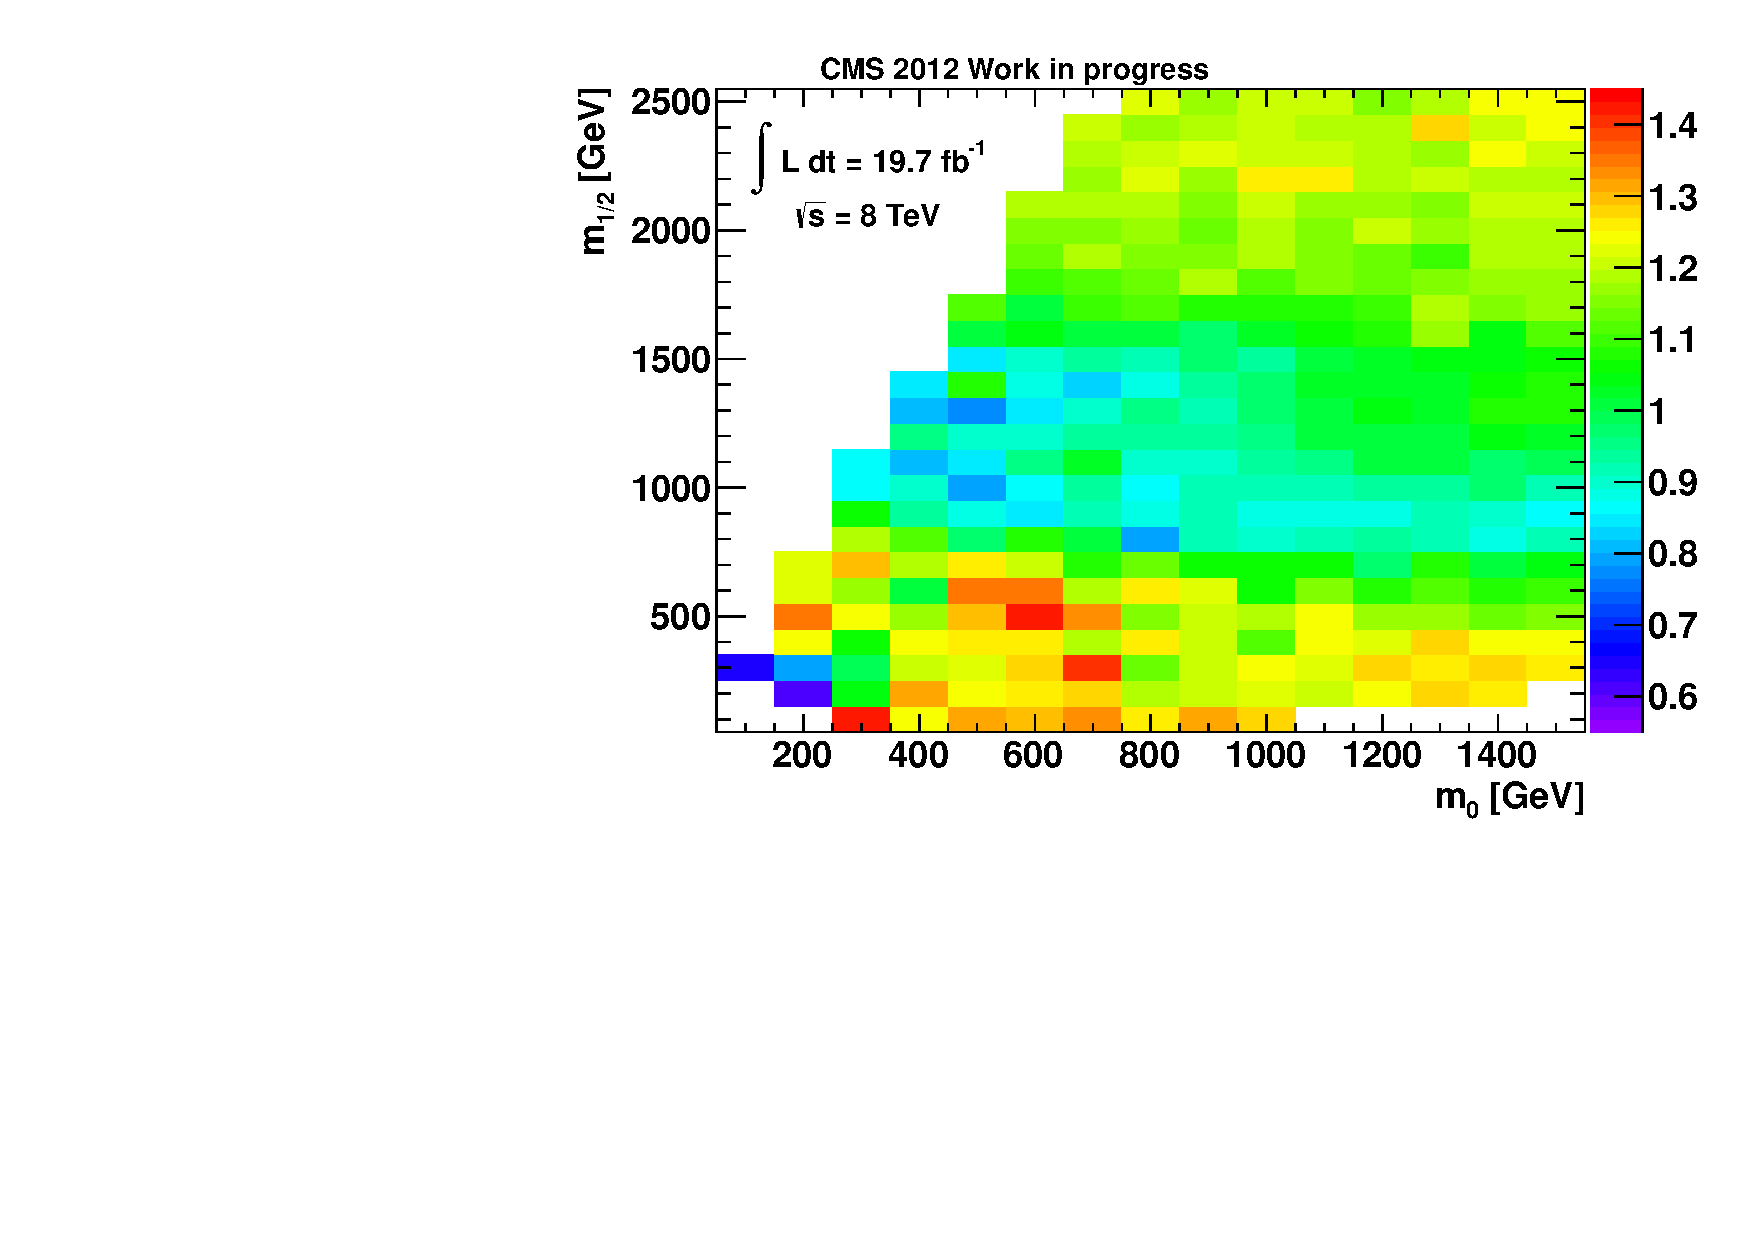
\includegraphics[width=0.7\textwidth]{plots/lambda_ratio.pdf}
  \caption{Ratio of the observed (\ref{fig:lambda-prime-obs}) to expected limits (\ref{fig:lambda-prime-exp}) for the model parameter $\lambda^{\prime}_{211}$.}
  \label{fig:lambda_ratio}
\end{figure}

Examining the ratio of expected and observed limits (Fig.~\ref{fig:lambda_ratio}), one can see that there are no rogue values deviating too much from the expectation. However, certain structures can be seen. They are the product of these mass parameters leading to certain smuon and gaugino masses, corresponding to one or two of the signal regions. Using the phase space point with $m_0 = 1000\,\text{GeV}, m_{1/2} = 1200\,\text{GeV}$ (Fig.~\ref{fig:final-dist}) as an example, one can see that its distribution has its main contribution in the SR 5 and 6, where data and MC are in reasonable agreement. Hence, the ratio for that region in phase space is roughly equal to 1. For $m_0 = 1000\,\text{GeV}, m_{1/2} = 200\,\text{GeV}$ on the other hand, the upward fluctuation of the measurement in the corresponding SR 4 leads to ratio of 1.1 or higher.


\section{Candidate Events}
\label{sec:candidate-events}

\begin{figure}[!htbp]
  \centering
  \begin{subfigure}[b]{0.75\textwidth}
    \centering
    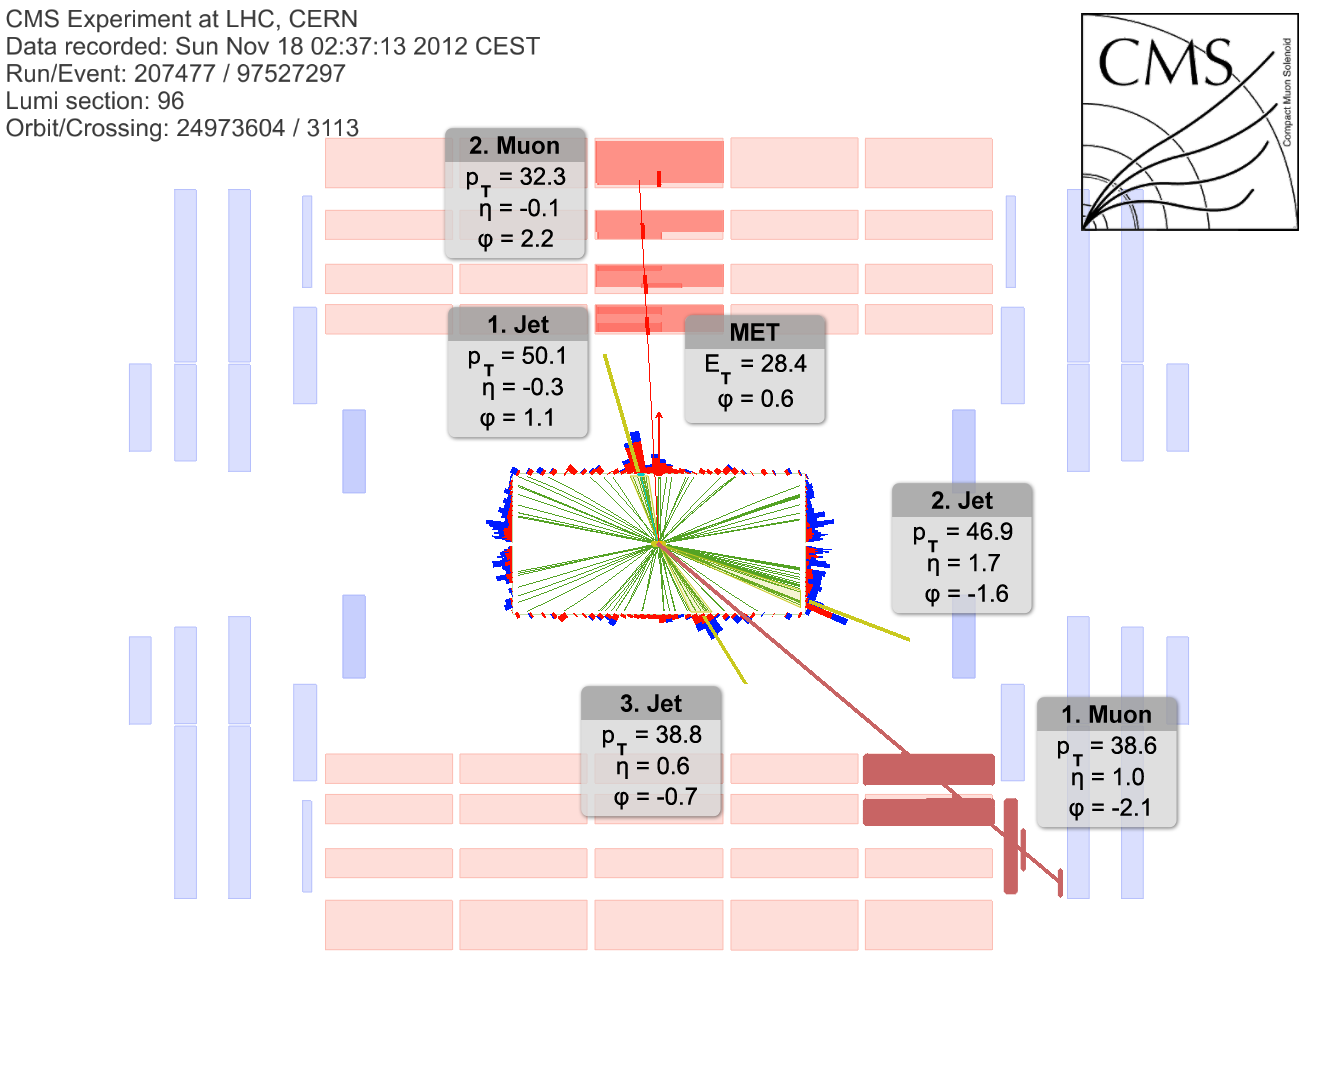
\includegraphics[width=\textwidth]{plots/event_display_eta_z.png}
    \caption{\label{fig:evt-eta-z}}
  \end{subfigure}
  \begin{subfigure}[b]{0.75\textwidth}
    \centering
    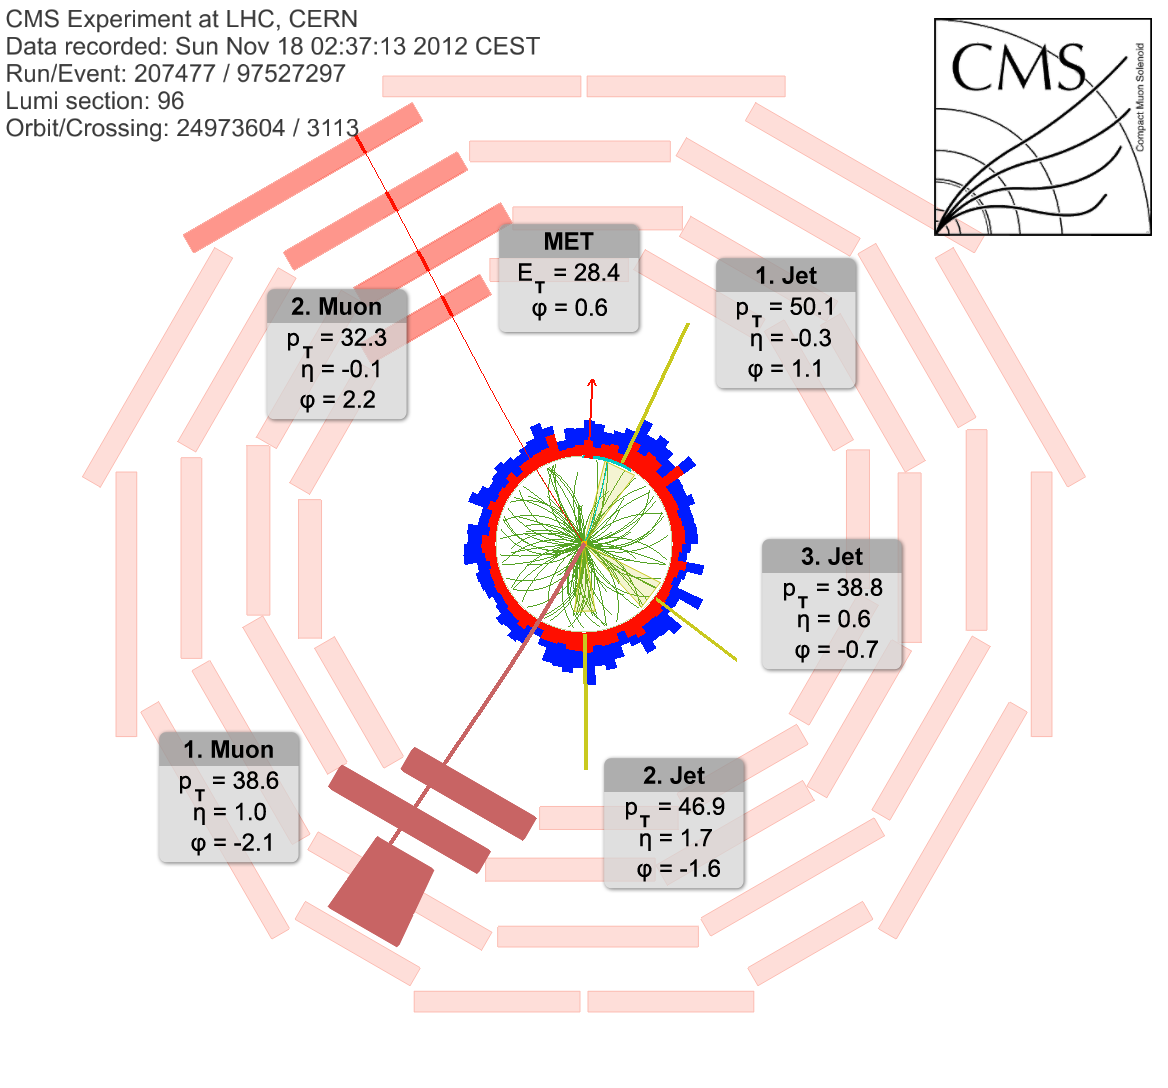
\includegraphics[width=\textwidth]{plots/event_display_phi_r.png}
    \caption{\label{fig:evt-phi-r}}
  \end{subfigure}
  \caption{Signal-like event candidate detected by the CMS. Shown are both the $\eta$-$z$- (\ref{fig:evt-eta-z}) and the $\phi$-$r$-plane (\ref{fig:evt-phi-r}).}
  \label{fig:evt-display}
\end{figure}

\noindent To summarize the event selection, an event that has been recorded by the CMS detector is being shown in figure~\ref{fig:evt-display}. Muons below the minimum transverse momentum of $20\,\text{GeV}$ and jets below the minimum energy of $30\,\text{GeV}$ have been removed. The event passed all selection requirements and visualizes the most important aspects of it. Both muons are highly energetic and well isolated, as they are reasonably separated from the various jets. The number of jets exceeds the minimum of two, while the respective jet's energy also surpasses the threshold by quite a margin. With the low amount of missing transverse energy that is needed to pass the upper limit of $50\,\text{GeV}$, the red arrow representing this quantity is barely noticeable.

\section{Conclusion and Outlook}
\label{sec:conclusion}

What has been presented, is a search for resonant production of second generation sleptons via single coupling dominance of the $\lambda^{\prime}_{211}$ parameter. For this purpose, the full $\mathcal{L} = 19.7\,\text{fb}^{-1}$ of double muon events recorded by the CMS experiment at proton-proton collisions with a center-of-mass energy of $\sqrt{s} = 8\,\text{TeV}$, is being used. The final state in question is composed of two reasonably well isolated, same-sign muons and at least two jets. An additional characteristic of the signature is a low amount of missing transverse energy, which is atypical for common SUSY events. As no significant excess of data has been observed in comparison to the Standard Model's prediction, the best limits to date have been set on the model parameter $\lambda^{\prime}_{211}$. They cover a range of up to $2.5\,\text{TeV}$ for the universal mass parameter of scalar particles $m_0$ and up to $1.5\,\text{TeV}$ for the universal mass parameter of fermionic particles $m_{1/2}$. A complementary expression through the mass of the smuon $m_{\tilde{\mu}}$ and gaugino $m_{\tilde{\chi}^0}$ in this model has also been provided.

For future efforts in this particular search, an improved selection efficiency for the signal could be achieved through taking the varying signature distributions of different RPV SUSY phase space points into account. This would require either fully flexible or individually adjusted thresholds for specific regions of the $m_0$-$m_{1/2}$-phase space.

Additional, easier to interpret results using ``simplified models'', based on the knowledge gained about the most important decay channels, are also possible and being investigated.

\section*{Acknowledgements} 
\label{sec:acknowledgements}

I offer my sincerest gratitude to both my family and my institute. Amongst the many people who helped me along the way, there are some which I would like to highlight. First of all, Professor Thomas Hebbeker, who enabled me to develop my thesis at his institute. Martin Weber, who supervised me throughout most of my work and introduced me to my new best friend ``Emacs''. Sebastian Th\"uer, who vigorously endured my constant nagging and questioning. Arnd Meyer, the voice of wisdom in times of need. Lars Sonnenschein, who was always eager to push for results. Andreas G\"ueth, miracle worker at the monstrosity called Monte Carlo generators. Daniel Teyssier, at efficiently working on efficiencies. My parents for allowing me to get this far and their omnipresent all around support. And everyone working at the institute, who all contribute to the work-oriented and yet relaxing atmosphere, allowing for an enjoyable experience throughout my time there.

%%% Local Variables: 
%%% mode: latex
%%% TeX-master: "document"
%%% End: 
